\documentclass[11pt]{article}
\usepackage[]{acl}
\usepackage{times}
\usepackage{latexsym}
\usepackage[T1]{fontenc}
\usepackage[utf8]{inputenc}
\usepackage{microtype}
\usepackage{inconsolata}
\usepackage{graphicx}
\graphicspath{{../results/figures/}{results/figures/}}

\title{Group 55 Progress Report:\\Predicting Bank Customer Churn}
\author{Mostafa Faghani, Musab Mondal\\
  \texttt{\{faghanim,mondam1\}@mcmaster.ca}}

\begin{document}
\maketitle

\section{Introduction}

When customers close their accounts, banks can lose future revenue and incur costs to acquire replacement customers. A churn model estimates which customers are most likely to leave so that a bank can prioritize outreach within a limited budget. False negatives represent missed opportunities to contact customers who leave, while false positives spend outreach resources on customers who would have stayed. Both errors matter when a retention offer carries a cost.

We treat churn prediction as supervised binary classification on tabular data. Each row describes one customer, and the model estimates the probability that the row's \texttt{Exited} label is one. We distinguish ranking customers by their scores from choosing a decision threshold for outreach. A bank with a fixed contact budget may care about the quality of the ranking, while the operating threshold determines how many customers receive an offer. In this milestone, we implement the proposed artificial neural network (ANN), compare it with a random forest and a majority baseline, and examine how the conclusions change with the metric.

\section{Related Work}

\citet{lemos2022} compared several classifiers on customer data from a Brazilian bank and found that random forests outperformed several alternatives on their evaluation. Their work motivates including a tree ensemble in our experiment. \citet{breiman2001} introduced random forests, which combine trees trained with randomness in their observations and feature choices. This offers a comparison with a model that learns interactions through sequential splits, while the ANN learns a representation through its hidden layers.

\citet{amuda2019} studied a multilayer perceptron for churn in a Nigerian financial institution and used dropout and L2 regularization. We begin with a smaller network and use this first run as a reference for later regularization experiments. Both banking studies used data from different institutions, so their published scores are context for choosing methods. The comparison in this report instead retrains each model on the same split of our dataset.

\citet{saito2015} show why precision-recall plots are informative when positive labels are uncommon. This is relevant here because accuracy can look high even when a model finds no churners. We report precision and recall at a fixed threshold and average precision across the ranked scores. We also report ROC AUC to compare discrimination under a second summary measure.

\section{Dataset}

We use the public \emph{Churn Modelling} dataset distributed through Kaggle \citep{churnData}. The supplied CSV has 10,000 customer records and 14 columns, including ten predictors, three identifiers, and the binary label \texttt{Exited}. The dataset supplies the labels, so this project uses the existing annotations. The sample includes 7,963 customers who stayed and 2,037 who exited, a churn prevalence of 20.37\% (Figure~\ref{fig:classes}).

\begin{figure}[t]
  \centering
  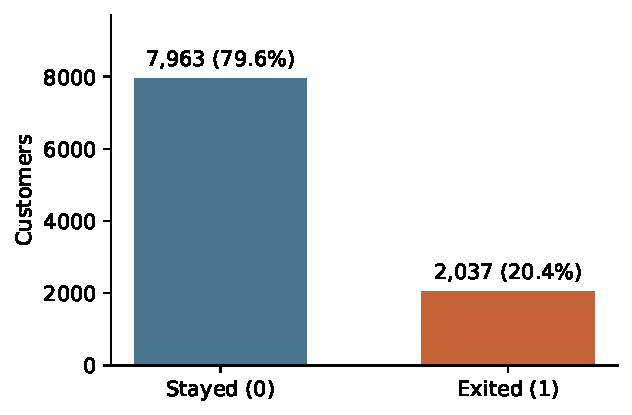
\includegraphics[width=\columnwidth]{class_distribution.pdf}
  \caption{Observed label distribution in the full dataset.}
  \label{fig:classes}
\end{figure}

We audited the file for missing cells, exact duplicate rows, repeated customer IDs, and repeated ten-feature records. All four counts were zero. The ages range from 18 to 92, credit scores from 350 to 850, tenure from zero to ten years, and recorded product counts from one to four. Both account flags contain only zero and one. The 3,617 zero-balance accounts were retained as observed values. We kept all records and used the supplied labels. The file does not provide a date or a follow-up window, which limits how precisely we can interpret the period covered by an exit.

The three recorded geographies are France (5,014 customers), Germany (2,509), and Spain (2,477). In this sample, 32.4\% of German customers exited, compared with 16.2\% in France and 16.7\% in Spain. Churn also differed by activity status, with 26.9\% of inactive and 14.3\% of active customers exiting. These are descriptive rates in the supplied records. They help explain why account activity and geography are reasonable predictors to evaluate, but they cannot establish what caused a customer to leave.

Product counts also show an association worth checking in later experiments. In this file, 7.6\% of customers with two products exited, compared with 27.7\% of customers with one product. All 60 customers recorded with four products exited. That group is small relative to the rest of the sample, so an apparent rule derived from it could be sensitive to a change in the customer population. For the preliminary experiment, we keep product count as a numeric input and let each model learn how to use it with the other fields.

\section{Features}

The model inputs are credit score, geography, gender, age, tenure, balance, number of products, credit-card ownership, active membership, and estimated salary. The preprocessing pipeline excludes row number, customer ID, and surname so that the model cannot use customer identifiers. It expands geography into one indicator per country and encodes the two recorded gender values as zero and one. The remaining fields pass through as numeric values. This produces a twelve-dimensional vector.

We fit the encoders and the standard scaler on the training records. The scaler applies the training means and standard deviations to the encoded vector, including the indicator columns. This puts the large monetary values and the smaller count and indicator values on comparable scales for the ANN. We apply the same fitted transformation to validation, test, and inference inputs. The random forest receives the same inputs for consistency across experiments, although its split decisions depend on feature ordering and generally need no scaling. The current models use all ten original predictors. The ANN learns hidden representations jointly with the classifier, and the experiment uses the observed class distribution without augmentation or resampling.

\section{Implementation}

\subsection{Artificial neural network}

The Keras model has two fully connected hidden layers with six units each and rectified linear unit activations. A single sigmoid output maps the final activation to a score in $(0,1)$ for the positive class. The network has 127 trainable parameters. The first layer can combine multiple input features, and the second can combine those intermediate activations into a representation for the final decision.

For an observed label $y$ and predicted probability $p$, the training objective is binary cross-entropy,
\[
  \ell(y,p) = -y\log p - (1-y)\log(1-p).
\]
The objective penalizes confident mistakes on either label. We train for 100 epochs with a batch size of 32 and use Adam, which adapts parameter updates using estimates of first and second gradient moments \citep{kingma2015}. The historical run uses the original architecture and training settings with a fixed seed. Adam uses learning rate 0.001, beta values 0.9 and 0.999, and epsilon $10^{-7}$. No dropout, explicit weight penalty, class weighting, or early stopping is used in this reference run. The average training loss decreased from 0.635 in the first epoch to 0.327 in the last (Figure~\ref{fig:training}). This curve shows optimization on the training set. Held-out performance is evaluated separately.

\begin{figure}[t]
  \centering
  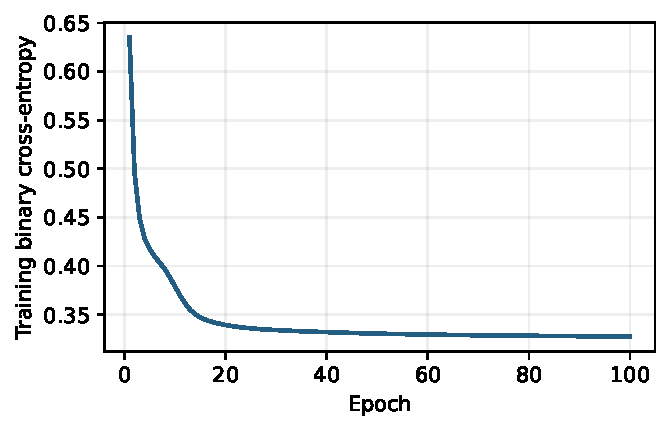
\includegraphics[width=\columnwidth]{ann_training_loss.pdf}
  \caption{ANN training binary cross-entropy over 100 epochs.}
  \label{fig:training}
\end{figure}

\subsection{Comparison models}

The majority baseline estimates the positive class probability as the fraction of churners in the training set, $1{,}426 / 7{,}000$. It returns this constant score for every record. At a cutoff of 0.5, this amounts to classifying every customer as staying. The baseline establishes how much apparent accuracy can be achieved using the class distribution alone.

The random forest trains 200 decision trees on bootstrap samples and uses Gini impurity when choosing splits. Each tree produces a class probability from its terminal leaf, and the forest averages those probabilities. It provides a learned comparison capable of using interactions among the same predictors. We use a fixed forest configuration for this milestone. The preliminary ANN and forest both train without class weighting.

\subsection{Reusable experiment workflow}

The training command selects a classifier from a registry and passes it to the experiment alongside a preprocessing pipeline. The Keras adapter exposes the same \texttt{fit} and \texttt{predict\_proba} methods as the other classifiers. The experiment handles the named input columns and extracts the probability of the positive class. Evaluation and figure generation then consume those probabilities, independently of how a classifier produced them.

Adding a classifier requires a factory for an estimator with the same interface. The train and evaluation splits, metric definitions, and plot generation can be reused, making model comparisons less prone to accidental changes in evaluation. Each saved pipeline includes the fitted encoder, scaler, and classifier so that a new record can be supplied in its original column format.

\section{Results and Evaluation}

\subsection{Protocol}

We stratify a single split by \texttt{Exited}, with 7,000 training, 1,500 validation, and 1,500 test records. These partitions have 1,426, 306, and 305 churners, respectively. The split and model seeds are zero. Both learned models and the baseline fit only on the training subset. The original repository run used validation for a preliminary check and recorded test results for the same fixed configurations. Table~\ref{tab:metrics} preserves those historical measurements. Because those test scores have already been inspected, this partition cannot serve as a fresh independent final evaluation after further tuning. New routine runs evaluate validation only; test evaluation now requires an explicit command-line option. The main comparison uses the shared decision rule $p>0.5$. We also examine a lower cutoff on validation to measure the effect on potential outreach volume.

Precision is the fraction of predicted churners who exited. Recall is the fraction of actual churners identified by the model. F1 is their harmonic mean. If the model predicts no positive labels, we report zero precision and F1. We also report accuracy, average precision (AP), and ROC AUC. AP summarizes precision across changes in recall as the threshold moves. The Brier score is the mean squared difference between predicted probabilities and observed labels. A lower Brier score indicates better squared probability error on the same data.

\begin{table*}[t]
  \centering
  \small
  \setlength{\tabcolsep}{7pt}
  \begin{tabular}{llrrrrrrr}
    \hline
    Split & Model & Accuracy & Precision & Recall & F1 & AP & ROC AUC & Brier \\
    \hline
    Validation & Majority & 0.796 & 0.000 & 0.000 & 0.000 & 0.204 & 0.500 & 0.162 \\
    Validation & ANN & 0.858 & 0.760 & 0.444 & 0.561 & 0.694 & 0.862 & 0.103 \\
    Validation & Random forest & 0.858 & 0.772 & 0.431 & 0.553 & 0.664 & 0.842 & 0.108 \\
    \hline
    Test & Majority & 0.797 & 0.000 & 0.000 & 0.000 & 0.203 & 0.500 & 0.162 \\
    Test & ANN & 0.844 & 0.680 & 0.439 & 0.534 & 0.676 & 0.853 & 0.108 \\
    Test & Random forest & 0.857 & 0.737 & 0.459 & 0.566 & 0.672 & 0.851 & 0.107 \\
    \hline
  \end{tabular}
  \caption{Validation and held-out test results. Accuracy, precision, recall, and F1 use the same 0.5 cutoff. AP, ROC AUC, and Brier use continuous scores.}
  \label{tab:metrics}
\end{table*}

\subsection{Preliminary findings}

On validation, the ANN and forest both reached 85.8\% accuracy. The ANN had higher average precision (0.694 versus 0.664) and slightly higher F1 (0.561 versus 0.553). On the test set, the random forest had higher F1 (0.566 versus 0.534), while the ANN had slightly higher average precision (0.676 versus 0.672). The test ranking curves in Figure~\ref{fig:pr} show how much precision can change as recall increases. Both learned models substantially exceed the no-skill AP of 0.203. The AP gap between them is small on this one split.

\begin{figure}[t]
  \centering
  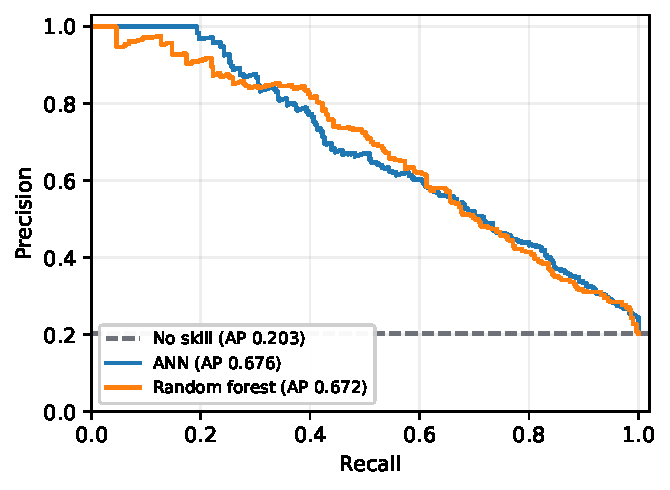
\includegraphics[width=\columnwidth]{test_precision_recall.pdf}
  \caption{Test precision-recall curves. The dashed line is the test churn prevalence and represents the no-skill reference for ranking.}
  \label{fig:pr}
\end{figure}

The majority baseline classified 79.7\% of test customers correctly while missing all 305 churners. The ANN identified 134 churners and flagged 63 customers who stayed. The random forest identified 140 churners and flagged 50 customers who stayed. This leaves 171 missed churners for the ANN and 165 for the forest (Figure~\ref{fig:confusion}). At the shared cutoff, each learned model still misses more than half of the positive cases.

\begin{figure*}[t]
  \centering
  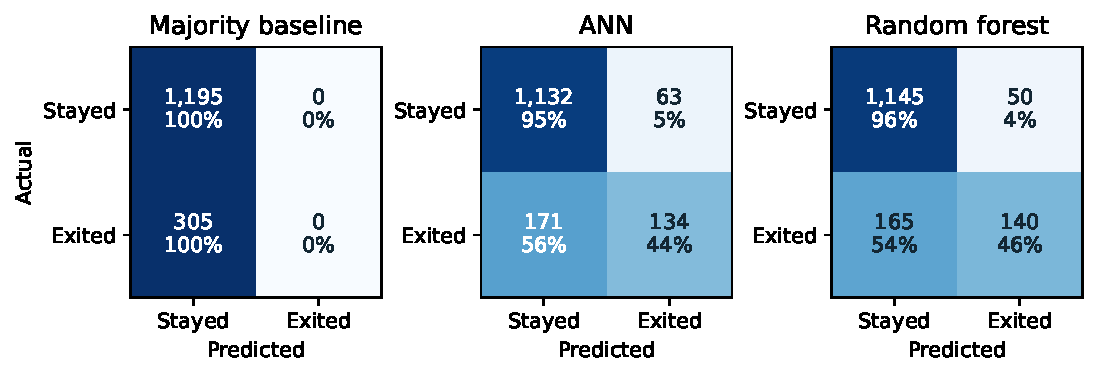
\includegraphics[width=0.92\textwidth]{test_confusion_matrices.pdf}
  \caption{Test confusion matrices at a 0.5 cutoff. Cells show counts and percentages within each actual class.}
  \label{fig:confusion}
\end{figure*}

Both learned models improved on the baseline Brier score in Table~\ref{tab:metrics}. The ANN had lower Brier error on validation, while the forest was slightly lower on test. Together with the reversal in F1 across splits, these differences show why we need more than one split before deciding which model to carry forward. This dataset also offers no out-of-time cohort, so the random holdout estimates performance on similar records from the supplied data.

\subsection{Validation threshold sensitivity}

As a separate check, we applied a cutoff of 0.30 to the validation predictions. At 0.50, the ANN identified 136 churners among 179 flagged customers. At 0.30 it identified 189 among 298 flagged customers. That adds 53 true positives and 66 false positives. Recall rose from 44.4\% to 61.8\%, while precision fell from 76.0\% to 63.4\%. The random forest showed the same trade-off. Its validation recall rose from 43.1\% to 66.0\%, while precision fell from 77.2\% to 59.4\%, and the number of flagged customers rose from 171 to 340.

These counts make the operating choice concrete. At 0.30, the forest identifies 13 more churners than the ANN, but flags 42 more people overall. If the bank could contact only 300 of these validation customers, the forest at this cutoff would exceed that budget. A comparison at a shared budget would be more informative than applying the same threshold to models whose scores have different distributions. The 0.30 check is exploratory, and Table~\ref{tab:metrics} retains 0.50 for all threshold-dependent results.


\subsection{Reproducibility and validation safeguards}

The revised runner rejects repeated customer identifiers, missing required fields, nonfinite numerical values, invalid account flags, and invalid negative account values before splitting. Numeric range checks are consistency checks rather than evidence of source authenticity. Each run records the data SHA-256, package versions, model parameters, row-level split assignments, and raw probabilities. An existing metrics file cannot be overwritten accidentally. Four automated tests cover split reproducibility and disjointness, duplicate-customer rejection, probability and threshold behavior, and preprocessing that remains fixed during inference. The forest uses two CPU workers while retaining its original tree settings.

\subsection{Extended development comparison}

The new comparison keeps the original twelve-dimensional inputs and seed-0 split. Logistic regression uses L2 regularization, $C=1$, and at most 1,000 L-BFGS iterations. XGBoost uses 300 depth-three trees, learning rate 0.05, row and feature subsampling of 0.8, and L2 regularization parameter 1. Its binary logistic objective uses regularized gradient boosting. These models are trained on the 7,000 training records only. Table~\ref{tab:extension} is generated directly from the new run's metrics rather than transcribed by hand. The original ANN results remain separately identified because they come from the earlier Keras run, not this comparison run.

\begin{table}[t]
\centering\small
\begin{tabular}{lrrrr}
\hline
Model & F1 & AP & AUC & Brier \\
\hline
Prior & 0.000 & 0.204 & 0.500 & 0.162 \\
logistic & 0.302 & 0.480 & 0.774 & 0.135 \\
Forest & 0.565 & 0.665 & 0.843 & 0.108 \\
xgboost & 0.575 & 0.694 & 0.863 & 0.103 \\
\hline
\end{tabular}
\caption{New validation-only comparison on the original seed-0 split. Threshold-dependent scores use $p>0.5$. This run does not evaluate test data.}
\label{tab:extension}
\end{table}


The extension is a development experiment, not a final model selection result. Its raw validation probabilities allow independent recomputation of every metric. Log loss is also exported, supplementing the Brier score. No additional test scores are produced. A validation gain cannot establish robustness across random splits, calibration, causal benefit from outreach, or superiority on another bank's customers.

\section{Feedback and Plans}

During the proposal consultation, we discussed model choice, the training/validation/test split, and how to evaluate churn when the classes are imbalanced. The TA recommended an ANN for this project and advised considering precision and recall alongside accuracy. We used the proposed 70/15/15 split, trained the ANN, and added a forest and majority comparison. The zero recall of the majority baseline illustrates why the evaluation includes both types of error.

The next priority is to select an operating threshold on validation data. We will compare recall at a fixed precision or outreach budget, because the default threshold misses more than half the churners. If the goal is to contact a fixed number of customers, we can measure precision and recall among the highest-scoring records at that budget. We will also compare unweighted and class-weighted training to see whether weighting improves ranking, changes the operating threshold, or both.

To compare probability estimates more directly, we will group validation scores into ranges and plot the observed churn fraction against the mean prediction in each range. The Brier score summarizes probability error, but it does not show where scores overestimate or underestimate observed churn. A useful outreach score may still need calibration before its numeric value can be interpreted as a probability. We will keep calibration and threshold selection on development data.

XGBoost \citep{chen2016} and logistic regression are now registered comparators, evaluated on the same development split. Their initial configurations are fixed rather than selected by a hyperparameter search. We also plan to repeat the comparison over stratified folds on the development records, inspect validation loss during ANN training, and use reliability plots to investigate probability calibration. Since the current test outcomes have been inspected for the milestone, an independent cohort would provide a stronger final check after tuning if one becomes available. Where sample sizes permit, we will also compare error rates by geography and gender and report subgroup counts alongside those rates.

\section*{Team Contributions}

\noindent\textbf{Musab Mondal} led the classifier implementation and ANN training, evaluation on the stratified split, comparison with the majority baseline and random forest, and preparation of the progress report and figures.

\noindent\textbf{Mostafa Faghani} cleaned the dataset, implemented encoding and scaling, and wrote the related work, dataset, features, and implementation sections.


\clearpage
\bibliography{custom}
\end{document}


